\documentclass{standalone}
\begin{document}
		\subsection{U-Net}
		
		Artificial Neural Networks are formed by using artificial neurons derived from physiological models~\cite{INP:Withey}. Neural Networks are made by nodes that simulate a biological learning. Each node of the network it is able to perform an elementary operation.  For imagery analysis are usually used Convolutional Neural Networks(CNN), also known as shift invariant or space invariant artificial neural networks (SIANN).\\
			
		In biological image processing usually is used the  so colled modelU-Net, which is a kind of convolutional neural network which allows to overcome the two main drawbacks of this kind of networks :
		\begin{itemize}
			\item Needs of a huge size fo training data
			\item Size of the considered network. 
		\end{itemize}
	
		That because, for medical and biological segmentation purposes, training dataset with a huge size are not available.\\
		Convolutional Networks usually are used nn classification tasks, which requires only one label. For biological and medical purposes, the segmentation 	should include localization and a class label should be assigned on each voxel.\\
		To achieve this purposes, in $2015$ for the ISB cell tracking challenge, Olaf Ronneberger, Philipp Fischer, and Thomas Brox have developed this kind of network~\cite{ART:Johannes}. \\
		This kind of network is a modification and simplification of a fully convolutional neural network, making it suitable to works with few training samples.
		The whole structure is divided into two main parts:
		\begin{itemize}
			\item Contraction path(\textit{encoder}) : sequence of convolutional and pooling layers, which aim
			to extract features and reduce the input dimensionality. 
			
			\item Expansion Path(\textit(decoder)) : second set of convolutional and up-sampling layers, to reconstruct the
			feature map size and the segmentation mask, which aims to process the extracted features
		\end{itemize}
		Decode path tends to lose some of the igher level features that the encoder learned: Using shortcut connection, the output of the encoding layers are directly passed to the decoder layer, preserving the important features~\cite{PhDtheis}.\\
	
		
		As I've said the network is composed by two path: the contractive path and the extractive path. The contracting path is a typical convolutional network that consists of repeated application of convolutions, each followed by a rectified linear unit (ReLU) and a max pooling operation. During the contraction, the spatial information is reduced while feature information is increased. The expansive pathway combines the feature and spatial information through a sequence of up-convolutions and concatenations with high-resolution features from the contracting path~\cite{ART:Johannes}.\\
		
		In particular the contractive path consist in the application of $3x3$ convolutions, each of them followed by a rectified linear unit(ReLU). and a 2x2 pooling operation. very step in the expansive path consists of an upsampling of the feature map followed by a 2x2 convolution (“up-convolution”) that halves the number of feature channels, a concatenation with the correspondingly cropped feature map from the contracting path, and two 3x3 convolutions, each followed by a ReLU. The cropping is necessary due to the loss of border pixels in every convolution. At the final layer a 1x1 convolution is used to map each 64-component feature vector to the desired number of classes
		
		\begin{figure}[h!]
			\centering
				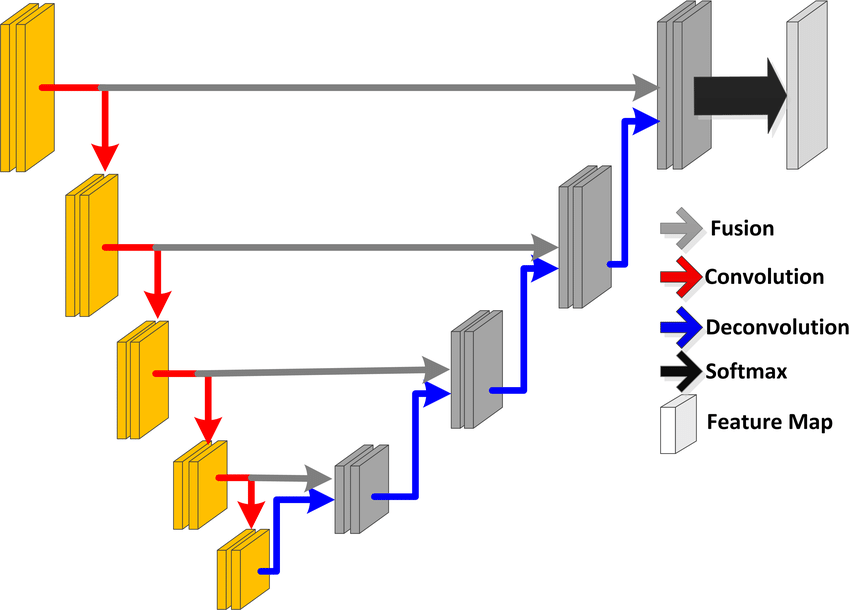
\includegraphics[scale=.4]{UNet.png}
					\caption{}\label{fig:UNet}
		\end{figure}
	
		One of the important modification of this network is that in the upsampling part  have also a large number of feature channels, which allow the network to propagate context information to higher resolution layers, as a consequence the expansive path is symmetric to the contractive one, making the U shape, as we can see in the structure diplayed in \figurename\,\ref{fig:UNet}. In a U-Net the segmentation map only contains the pixels for which the full context is available~\cite{ART:Johannes}.\\
		In order to work with few training data, this network makes a huge data augmentation, by applying an elastic deformation to the training images, that allow the network to learn invariance to such kind of transformation. 
. 
\end{document}